\documentclass[11pt]{article}
\usepackage{hyperref,array,graphicx,caption,geometry}
\usepackage[french]{babel}
\title{TEXT FORMATTING in \LaTeX}
\author{Mohamed EL-BADRI}
\date{\today}

\begin{document}
\section{INTRODUCTION}
	\subsection{Définition}
Les prévisions saisonnières sont souvent présentées sous forme de « probabilités en terciles », qui font référence à la
probabilité que l’on puisse s’attendre à ce que les conditions soient supérieures à la
normale, normales ou inférieures à la normale. Les valeurs supérieures et inférieures à la normale ne sont pas des catégories extrêmes, chacune constituant un événement
sur 3 ans. Ces catégories sont définies en fonction des précipitations
observées historiquement. Sans prévision saisonnière, nous supposons qu’il y a une chance égale que
les conditions tombent dans l’une des trois catégories ; ainsi, il y a 33 \% de chances que l’un de ces résultats soit atteint.


\vspace{0.3cm}


Les prévisions saisonnières utilisent des modèles climatiques pour prédire à quoi pourraient ressembler un paramètre, par exemple les précipitations saisonnières
et cette prédiction se reflète dans les prévisions en faisant pencher les probabilités
(en augmentant la probabilité) en faveur de l'un de ces résultats ; par exemple,
les modèles de prévision peuvent indiquer plus de pluie que d'habitude. Ces informations peuvent être
utilisées pour augmenter la probabilité du résultat « supérieur à la normale » de 33 \% à 45 \% ;
cependant, si la probabilité d'un résultat « supérieur à la normale » est de 45 \%, il existe toujours 55 \% de chances
que ce résultat ne soit pas supérieur à la normale.
	\subsection{prévision saisonnière | prévision déterministe}
		\begin{table}[h!]
		\centering
			\begin{tabular}{|>{\centering\arraybackslash}p{7cm}|>{\centering\arraybackslash}p{7cm}|}
				\hline
				\textbf{PRÉVISION SAISONNIÈRE} & \textbf{PRÉVISION DÉTERMINISTE}.\\ 					
				\hline
				Information sur la situation moyenne de la saison & Information sur chaque jours.\\ 
				\hline
				Prévision sur une large région & Prévision avec une résolution 					élevée.\\
				\hline
				Information sous forme de probabilités & Information définitive.\\
				\hline
			\end{tabular}
		\caption{Comparaison entre la Prévision saisonnière et la déterministe}
		\end{table}
		
		
	\subsection{Principe de la prévision saisonnière.}
		la prévision saisonnière est faire sur une échéance plus éloignée que la prévision déterministe (généralement de 3 à 6 mois). Cette prévisoion est en faite possible grâce aux indicateurs climatiques qui sont liée à l'océon de facon générale. la capacité calorifique elevé de l'eau permet un changement plus lent de la température des océans ce qui les permet de maintenir la chaleur pour plusieurs mois. Donc cet aspect aide à la prévision de la situation dans quelques mois mais avec une résolution spatiale et temporelles plus large.\\
		Aussi on peut opter pour l'ENSO par exemple pour avoir une idée sur la situation de température et de précipitation dans quelques mois. Cela pose une question importante, est ce que toutes les régions dans le monde sont également prédictibles? \\ 
		la réponse est tout simplement non, généralement les régions tropicales sont les plus prédictibles grâce à la forte connexion de cette région avec les indicateurs climatiques.   \\

\begin{figure}[h]
    \centering
    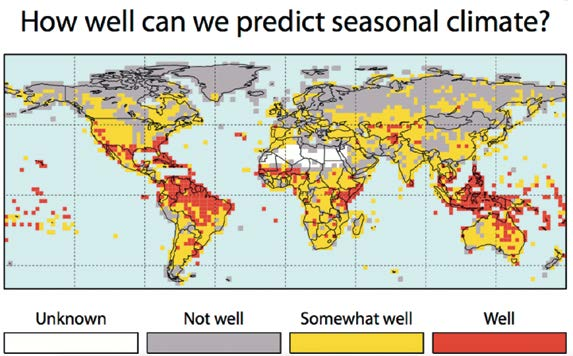
\includegraphics[scale=0.5]{REGIONS_PREDICTIBILITY.png}
    \caption*{Prédictibilité des Régions.\footnotemark{} }
\end{figure}
\footnotetext{International Research Institute for Climate and Society}.



\end{document}